\documentclass[generalized_symmetry.tex]{subfiles}
\setcounter{chapter}{3}
\begin{document}

\chapter{高次形式対称性}
これまでは主に2次元の一般化対称性について見てきましたが、ここから徐々に高次元の一般化対称性について見ていくことにします。まずは、高次元での高次形式対称性と呼ばれるクラスの一般化対称性について見ていきます。

\section{高次形式対称性の定義}

まず$p$形式対称性を定義します。群を$G$があって、$g\in G$と時空内の余次元$p+1$の向きのついた面$M$があったときに$M$に局在したトポロジカル欠陥$U_g(M)$が存在して、次の条件を満たすとき、これを$p$形式対称性と呼びます。
\begin{enumerate}
    \item フュージョン則は群の積になります。
    \begin{align}
        \orientedline{U_g}
        \orientedline{U_h}
        =
        \orientedline{U_{gh}}
    \end{align}
    \item 単位元、逆元も群の構造に従います。つまり
    \begin{align}
        U_1(M) = 1, \quad U_{g^{-1}}(M) = U_g(-M)
    \end{align}
\end{enumerate}
この言葉遣いでは$0$形式対称性は普通の対称性です。$p>0$のとき$p$形式対称性は高次形式対称性と呼ばれます。高次形式対称性の場合には、トポロジカルな変形でフュージョンの順番を入れ替えることができるので、群$G$はアーベル群になります。

次に、$p$形式対称性の欠陥(演算子)への作用について見ていきましょう。一般に$p$形式対称性は$p$次元の欠陥に自然に作用します。例えば普通の対称性は$0$形式対称性ですから、$0$次元の欠陥である局所演算子に自然に作用します。もう少し正確に述べます。$C$を次元$p$の曲面として$W_a(C)$を$C$に局在した次元$p$の(トポロジカルとは限らない)欠陥とします。ここで$a$はラベルです。余次元$p+1$の曲面$M$を$C$に絡み数1で絡んでいる曲面として$U_g(M)$は$W_a(C)$に次のように作用します。
\begin{align}
    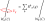
\includegraphics{actionp-formsym.pdf}.
\end{align}
ここで$R^{b}{}_{a}(g)$は$G$の表現行列です。高次形式対称性の場合には$G$はアーベル群でしたから、既約表現は1次元です。つまり、$R^{b}{}_{a}(g)=$(位相)$\delta^{b}_{a}$となる基底をとることができます。

\section{格子ゲージ理論の中心対称性}
\section{背景ゲージ場その1}
\section{背景ゲージ場その2:単体コホモロジー}
\section{自発的対称性の破れ}


\end{document}